\chapter{Heat: Where Every Watt Ends Up}
\label{ch:heat}

A chip does useful work, but physically, all the electrical energy it consumes turns into heat. A GPU drawing 700\,W is, from the room's point of view, a 700\,W heater. Getting that heat out without letting the chip overheat is a major part of hardware engineering, and candidates have reported assessment questions on heat sinks. This chapter explains how heat moves, how to calculate a chip's temperature, and why heat sinks are built the way they are.

\section{Every watt becomes heat}

Energy is never destroyed, only converted. When current flows through the resistance of wires and transistors, electrical energy becomes heat (Chapter~\ref{ch:electricity}). Charging and discharging capacitance also turns energy into heat in the transistors that do the charging (Chapter~\ref{ch:power}). The chip stores almost none of this energy, so in steady operation:
\[
  \text{heat produced per second} = \text{electrical power consumed}.
\]

What makes chips hard to cool is not just total power but \term{power density}: power per unit area. A large GPU die is roughly 8\,cm$^2$. At 700\,W that is close to 90\,W/cm$^2$, many times the power density of a kitchen stove burner, concentrated in a sliver of silicon smaller than a postage stamp.

\section{Why temperature matters}

Silicon chips are typically allowed to run up to a maximum \term{junction temperature} (the temperature of the transistors themselves) of around 100 to 110\,\textdegree C, depending on the product. Staying below that limit matters because temperature affects nearly everything:

\begin{itemize}
  \item \textbf{Leakage power rises steeply with temperature} (Chapter~\ref{ch:power}). Hotter chips waste more power even when idle, which makes them hotter still.
  \item \textbf{Speed changes.} In most conditions transistors and wires get slower when hot (Chapter~\ref{ch:pvt}).
  \item \textbf{Aging speeds up.} Wear-out mechanisms such as electromigration (Chapter~\ref{ch:fab}) accelerate strongly with temperature. A common rule of thumb is that many failure rates roughly double for every 10\,\textdegree C rise.
\end{itemize}

\section{The three ways heat moves}

\begin{itemize}
  \item \term{Conduction}: heat flows through a solid (or still fluid) from hot to cold, passed along by vibrating atoms and moving electrons. This is how heat gets from the transistors, through the silicon and metal, to the heat sink.
  \item \term{Convection}: a moving fluid (air or liquid) picks up heat from a surface and carries it away. This is how a heat sink hands its heat to the air. A fan makes it \emph{forced} convection, which is far more effective than air drifting on its own (\emph{natural} convection).
  \item \term{Radiation}: hot objects emit infrared light. For chips at normal temperatures this is a small effect, and we will ignore it.
\end{itemize}

\section{Thermal resistance: Ohm's law for heat}

Heat flow behaves just like current in a circuit, which gives us a powerful shortcut:

\begin{center}
\begin{tabular}{ll}
\toprule
Electrical & Thermal \\
\midrule
Current $I$ (A) & Heat flow $P$ (W) \\
Voltage difference $V$ (V) & Temperature difference $\Delta T$ (\textdegree C) \\
Resistance $R$ ($\Omega$) & Thermal resistance $\theta$ (\textdegree C/W) \\
$V = IR$ & $\Delta T = P\,\theta$ \\
\bottomrule
\end{tabular}
\end{center}

\begin{bigidea}
Temperature rise equals power times thermal resistance: $\Delta T = P\,\theta$. A thermal resistance of 0.2\,\textdegree C/W means every watt flowing through it raises the temperature difference across it by 0.2\,\textdegree C.
\end{bigidea}

Heat leaving a chip passes through a chain of layers, one after another, so their thermal resistances add in series exactly like resistors (Figure~\ref{fig:thermalstack}).

\begin{figure}[h]
\centering
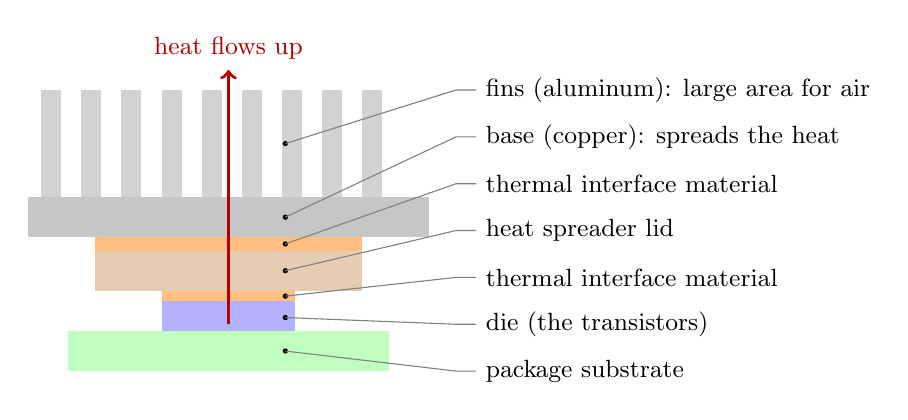
\begin{tikzpicture}[scale=0.85]
  % fins and base
  \foreach \x in {0.2,0.8,...,5.6} \fill[gray!35] (\x,3.4) rectangle (\x+0.3,5.0);
  \fill[gray!45] (0,2.8) rectangle (6,3.4);
  \fill[orange!50] (1.0,2.6) rectangle (5.0,2.8);
  \fill[brown!40] (1,2.0) rectangle (5,2.6);
  \fill[orange!50] (2,1.85) rectangle (4,2.0);
  \fill[blue!30] (2,1.4) rectangle (4,1.85);
  \fill[green!25] (0.6,0.8) rectangle (5.4,1.4);
  \draw[->,very thick,red!70!black] (3,1.5) -- (3,5.3) node[above]{\small heat flows up};
  % labels with leader lines
  \foreach \y/\ly/\t in {4.2/5.0/{fins (aluminum): large area for air},
                     3.1/4.3/{base (copper): spreads the heat},
                     2.7/3.6/{thermal interface material},
                     2.3/2.9/{heat spreader lid},
                     1.92/2.2/{thermal interface material},
                     1.6/1.5/{die (the transistors)},
                     1.1/0.8/{package substrate}} {
    \fill[black] (3.85,\y) circle (0.04);
    \draw[gray] (3.85,\y) -- (6.4,\ly) -- (6.7,\ly);
    \node[anchor=west,font=\small] at (6.7,\ly) {\t};}
\end{tikzpicture}
\caption{The path heat takes from the transistors to the air. Each layer adds thermal resistance.}
\label{fig:thermalstack}
\end{figure}

The standard names are:
\begin{itemize}
  \item $\theta_{jc}$: junction to case (from the transistors, through the die and lid).
  \item $\theta_{cs}$: case to sink (through the thermal interface material).
  \item $\theta_{sa}$: sink to ambient (from the heat sink into the surrounding air).
\end{itemize}
\[
  T_{\text{junction}} = T_{\text{ambient}} + P\,(\theta_{jc} + \theta_{cs} + \theta_{sa}).
\]

\begin{worked}{junction temperature}
A 300\,W chip has $\theta_{jc} = 0.05$, $\theta_{cs} = 0.03$ and $\theta_{sa} = 0.10$\,\textdegree C/W. The air entering the heat sink is at 35\,\textdegree C. What is the junction temperature?

Total thermal resistance: $0.05 + 0.03 + 0.10 = 0.18$\,\textdegree C/W. Temperature rise: $300 \times 0.18 = 54$\,\textdegree C. Junction temperature: $35 + 54 = 89$\,\textdegree C.
\end{worked}

\begin{worked}{sizing a heat sink}
The same chip must stay below 95\,\textdegree C with 40\,\textdegree C air. What is the largest $\theta_{sa}$ the heat sink may have?

Allowed rise: $95 - 40 = 55$\,\textdegree C. Allowed total resistance: $55/300 \approx 0.183$\,\textdegree C/W. Subtract the fixed parts: $0.183 - 0.05 - 0.03 = 0.103$\,\textdegree C/W. The heat sink and fan must achieve about 0.10\,\textdegree C/W or better.
\end{worked}

\section{Conduction and materials}

How well a material conducts heat is its \term{thermal conductivity} $k$, in W/(m$\cdot$K). A slab of thickness $L$ and area $A$ has thermal resistance
\[
  \theta = \frac{L}{k A},
\]
the same form as electrical resistance $R = \rho L / A$. Thin, wide layers of high-$k$ material are best.

\begin{center}
\begin{tabular}{lrl}
\toprule
Material & $k$ (W/(m$\cdot$K)), approx. & Notes \\
\midrule
Copper & 400 & excellent conductor; heavy, costly \\
Aluminum & 205--237 & about half of copper; light, cheap, easy to shape \\
Silicon & 150 & the die itself conducts well \\
Thermal paste & 1--10 & far worse than metal, but far better than air \\
Water (still) & 0.6 & poor conductor when not moving \\
Air (still) & 0.026 & a very good insulator \\
\bottomrule
\end{tabular}
\end{center}

\section{Heat sinks}

A heat sink has one job: take heat that is concentrated in a small area and spread it over a very large surface that moving air can touch. Its design follows from the two steps it performs.

\paragraph{Spreading (conduction).} The base sits on the chip and must carry heat sideways and upward quickly, without large temperature differences across it. This calls for high thermal conductivity, which is why bases are often copper. Many heat sinks also use \term{heat pipes} or \term{vapor chambers}: sealed copper tubes or plates containing a little liquid. The liquid boils at the hot end, the vapor rushes to the cold end and condenses, and the liquid wicks back. Moving heat by evaporation and condensation gives an effective conductivity far higher than solid copper.

\paragraph{Dumping (convection).} The \term{fins} give a large surface area to the air. Convection is roughly proportional to surface area, so more fins (or taller, thinner ones) remove more heat, up to the point where fins are so close that air cannot flow between them. A fan forces air through the fins and greatly lowers $\theta_{sa}$.

\paragraph{Why combine copper and aluminum?} Copper conducts heat about twice as well as aluminum, but it is about 3.3 times as dense (8.96 versus 2.70\,g/cm$^3$), costs more, and is harder to form into thin fins. A heat sink made entirely of copper would be very heavy and expensive. So a common design uses copper where heat is concentrated and conduction matters most (the base and heat pipes), and aluminum where large area matters most (the fins). Each metal goes where its strength counts.

\begin{onoa}
Candidates have reported multiple-choice questions on heat sinks. The ideas to have ready: fins increase surface area for convection; fans lower the sink-to-air thermal resistance; copper conducts better but is heavier and costlier than aluminum, so the two are combined; heat pipes move heat by phase change; and thermal paste fills air gaps.
\end{onoa}

\section{Thermal interface materials}

Two metal surfaces that look flat are rough at the microscopic scale. Pressed together, they touch only at high points, leaving tiny gaps filled with air, and air is an excellent insulator. A \term{thermal interface material} (TIM), such as thermal paste, a pad, or a soldered metal layer, fills those gaps.

TIM conducts heat much worse than metal, so it should be as thin as possible: just enough to fill the gaps. Too much paste adds thermal resistance instead of removing it.

\section{Air versus liquid cooling}

The heat a moving fluid carries away is
\[
  P = \dot m\, c\, \Delta T,
\]
where $\dot m$ is the mass flow rate (kg/s), $c$ the \term{specific heat} (energy to warm 1\,kg by 1\,\textdegree C), and $\Delta T$ how much the fluid warms up. Water's specific heat is about 4.18\,J/(g$\cdot$K), about four times air's (about 1.0), and water is roughly 800 times denser. Per unit volume, water carries several thousand times more heat per degree than air.

\begin{worked}{removing 1000\,W}
How much water, and how much air, must flow to carry away 1000\,W while warming by 10\,\textdegree C?

Water: $\dot m = 1000/(4180 \times 10) \approx 0.024$\,kg/s, about 1.4 liters per minute: a gentle trickle.

Air: $\dot m = 1000/(1005 \times 10) \approx 0.10$\,kg/s. At about 1.2\,kg/m$^3$, that is about 0.083\,m$^3$/s, or 83 liters every second: a powerful fan.
\end{worked}

This is why the highest-power data-center GPU systems are increasingly liquid cooled: air simply cannot move enough heat through a small space.

\section{Thermal throttling and runaway}

Chips contain on-die temperature sensors. When the temperature approaches the limit, power-management firmware lowers the clock frequency and supply voltage. Because dynamic power is proportional to $V^2 f$ (Chapter~\ref{ch:power}), even a modest reduction cuts power, and therefore heat, sharply. This is \term{thermal throttling}.

\term{Thermal runaway} is the dangerous loop in the other direction: higher temperature raises leakage power, which raises temperature, which raises leakage further. A cooling system must have enough margin that this loop settles instead of running away.

\section{Summary}

\begin{itemize}
  \item All the power a chip consumes becomes heat; power density is what makes cooling hard.
  \item Heat moves by conduction, convection and radiation (the last is minor for chips).
  \item $\Delta T = P\,\theta$; thermal resistances in the heat path add in series.
  \item Heat sinks spread heat (conduction: copper base, heat pipes) and dump it (convection: large fin area, fans).
  \item Copper conducts better but is heavy and costly; aluminum is light and cheap; good designs combine them.
  \item TIM replaces insulating air gaps; it should be thin.
  \item Liquid carries far more heat per volume than air.
\end{itemize}

\section{Exercises}

\begin{enumerate}
  \item A 250\,W chip has a total junction-to-ambient thermal resistance of 0.2\,\textdegree C/W in 25\,\textdegree C air. Find its junction temperature.
  \item A 400\,W chip must stay below 95\,\textdegree C in 40\,\textdegree C air. What is the maximum total thermal resistance allowed?
  \item Why do many heat sinks use a copper base with aluminum fins rather than one metal throughout?
  \item Why is thermal paste needed between a chip and its heat sink, and why should the layer be thin?
  \item True or false: adding fins to a heat sink increases its thermal resistance.
  \item A chip is overheating. Its firmware lowers the supply voltage by 10\% and the clock frequency by 10\%. By roughly what percentage does dynamic power fall?
  \item Explain thermal runaway in one or two sentences.
\end{enumerate}

\subsection*{Answers}
\begin{enumerate}
  \item $T_j = 25 + 250 \times 0.2 = 75$\,\textdegree C.
  \item $(95 - 40)/400 = 0.1375$\,\textdegree C/W.
  \item Copper conducts heat about twice as well, which matters most where heat is concentrated (the base). But copper is about 3.3 times denser and more expensive, so the large fin area is made of light, cheap aluminum. Each material is used where it helps most.
  \item Microscopic roughness leaves air gaps, and air insulates. Paste fills the gaps. Paste conducts much worse than metal, so a thick layer adds resistance; it should be just thick enough to fill the gaps.
  \item False. Fins add surface area for convection, which lowers the sink-to-air thermal resistance.
  \item Power scales with $V^2 f$: $0.9^2 \times 0.9 = 0.729$, so power falls by about 27\%.
  \item Higher temperature increases leakage power, which produces more heat and raises temperature further. If cooling cannot keep up, the loop keeps escalating.
\end{enumerate}
